\tableofcontents

\newpage
%\section{Introducción}

\section{Historia}
La idea de Kotlin se concibió en el 2010 en la compañía JetBrains\footnote{\url{https://www.jetbrains.com/}}, fabricantes de herramientas de desarrollo para muchos lenguajes incluido \texttt{Java}, \texttt{C\#}, \texttt{JavaScript}, \texttt{Python}, \texttt{Ruby} y \texttt{PHP}\cite{kotlin-in-action}. El Proyecto Kotlin fue revelado en Julio del 2011. Era un nuevo lenguaje para la \emph{Java Virtual Machine} (JVM) que había estado en desarrollo por un año\cite{krill}. Dentro de la compañía se acusaba que muchos lenguajes de programación no contaban con las características que ellos estaban buscando, con la excepción de \texttt{Scala}, pero el lento tiempo de compilación de \texttt{Scala} era una deficiencia obvia. Uno de los objetivos de \texttt{Kotlin} era contar con un tiempo de compilación tan rápido como en el de \texttt{Java}.

De acuerdo con Dmitry Jemerov, ingeniero en Jetbrains \cite{kotlin-in-action}: 

\emph{``La experiencia en la construcción de herramientas para una conjunto diverso de lenguajes nos ha dado una perspectiva y entendimiento único en el diseño de lenguajes pero, a pesar de esto varios de nuestros entornos de desarrollo estaban construidos en Java. Teníamos cierta envidia de nuestro equipo de .Net quienes desarrollaban en \texttt{C\#}, un lenguaje rápido, moderno y de rápida evolución. Pero no encontrábamos ningún lenguaje que pudiéramos usar en lugar de Java.}

\emph{¿Cuáles eran nuestro requerimientos para este lenguaje? Lo primero y lo más obvio era tipos estáticos. No conocemos ninguna otra forma de desarrollar miles de millones de líneas de código sin volvernos locos. Segundo, necesitábamos total compatibilidad con el código Java existente. El código es un gran activo para JetBrains, y no nos podíamos permitir perderlo o devaluarlo debido a dificultades en interoperatibilidad. En tercer lugar, no queríamos aceptar ningún compromiso en términos de calidad de herramientas. La productividad del desarrollador es el valor más importante para una compañía como JetBrains, y el contar con buenas herramientas es esencial para lograr esto. Por último, necesitábamos un lenguaje que fuera fácil de leer y de razonar. Con esto en mente nos decidimos a embarcarnos en un proyecto para crear un nuevo lenguaje: Kotlin''.}

\texttt{Kotlin v1.0} fue lanzado en Febrero del 2016\cite{kotlin-v1}. En Google \texttt{I/O} 2017, Google anunció soporte para \texttt{Kotlin} en \texttt{Android}\cite{kotlin-in-android}. \texttt{Kotlin v1.2} se lanzó en Noviembre del 2017. Compartir código entre la JVM y \texttt{JavaScript} fue una característica agregada a esta version\cite{kotlin-v12}.

Kotlin lleva el nombre de una isla cerca de San Petersburgo\footnote{\url{https://en.wikipedia.org/wiki/Kotlin_Island}}, Rusia, donde se encuentra la mayor parte del equipo de desarrollo de Kotlin\cite{kotlin-in-action}.



\section{Características del Lenguaje}

\subsection{Valores y tipos de datos base}
En Kotlin, todo es un objeto en el sentido que se pueden invocar funciones y propiedades en cualquier variable. Algunos de los tipos pueden tener una representación interna especial (por ejemplo, números, caracteres y booleanos pueden ser representados como tipos primitivos en tiempo de ejecución) pero que para el usuario lucen como una clase ordinaria. 

\subsubsection{Números}
Kotlin proporciona las siguientes tipos para representar números:
\begin{verbatim}
    Double 64bit, Int 32bit, Float 32bit, Short 16bit, Long 64bit, Byte 8bit
\end{verbatim}

%\begin{table}[h]
%    \centering
%    \begin{tabular}{cr||cr||cr}
%        \toprule[1.5pt]
%        \textbf{Tipo} & \textbf{Bit} & \textbf{Tipo} & \textbf{Bit} & \textbf{Tipo} & \textbf{Bit} \\
%        \midrule
%            {\tt Double} & $64$ & {\tt Float} & $32$ & {\tt Long} & $64$\\
%            {\tt Int} & $32$ & {\tt Short} & $16$ & {\tt Byte} & $8$\\
%        \bottomrule[1.5pt]
%    \end{tabular}
%\end{table}

\subsubsection{Caracteres}
Son representados por el tipo \texttt{Char}. No pueden ser tratados directamente como números. Los literales van en comillas simples: \texttt{'1'}. Caracteres especiales pueden ser escapados usando un \emph{backslash}. Las siguientes secuencias de escape son soportadas: 
\begin{verbatim}\t, \b, \n, \r, \', \", \\, \$
\end{verbatim}

\subsubsection{Booleanos}
El tipo \texttt{Boolean} representa booleanos y tiene dos tipos \texttt{true} y \texttt{false}.

\subsubsection{Arrays}
Los \emph{Arrays} en Kotlin se representan por la clase \texttt{Array}, que tiene la propiedad \texttt{size} y funciones \texttt{get}, \texttt{set}, entre otras que son útiles para trabajar con este tipo de estructura.

\subsubsection{Strings}
Se representan con la clase \texttt{String}. Los \emph{String} son inmutables. Los elementos de un \texttt{String} son caracteres que puede ser accedidos por la operación de indexación \texttt{s[i]}. Un \texttt{String} puede ser recorrido por medio de un ciclo \texttt{for-loop}.

\subsubsection{String Literals}
Kotlin tiene dos tipo de \emph{string literals}: \emph{strings} escapados que pueden tener caracteres escapados en él y \emph{strings} crudos (\emph{raw}) que pueden contener varias líneas y texto arbitrario.
\begin{verbatim}
    val s = "Hello, world!\n"
    val text = """
        for (c in "foo") 
            print(c)
    """
\end{verbatim}

\subsubsection{String Templates}
Los \emph{strings} pueden contener expresiones emplantilladas, piezas de código que puede ser evaluadas y cuyos resultados se concatenan dentro del \emph{string}. 
%% cambiar \$i por $i
\begin{verbatim}
    val i = 10
    print("i = \$i") //imprime "i = 10"
\end{verbatim}



%\lstset{framexleftmargin=5mm, frame=shadowbox, rulesepcolor=\color{blue}}
%\begin{lstlisting}[language=Java]
%fun main(args: Array<String>) {
%    println("Hello, world!")
%}
%\end{lstlisting}

\subsection{Variables y almacenamiento} \label{sec:variables-almacenamiento}
Para declarar una variable en Kotlin, se inicia con el nombre del identificador se puede o no poner el tipo luego del nombre
\begin{verbatim}
    val question = "The Ultimate Question of Life, the Universe, and Everything"
    val answer: Int = 42
\end{verbatim}
Si no se especifica el tipo, el compilador analiza la expresión y su inicializador, y usa el tipo como el tipo de variable\cite{kotlin-in-action}. En el ejemplo anterior, \texttt{42}, el inicializador tiene un tipo \texttt{Int}, por lo tanto la variable va a tener el mismo tipo. Si la variable no se inicializa, se necesita especificar su tipo explícitamente:
\begin{verbatim}
    val answer: Int
    answer = 42
\end{verbatim}

Existen dos palabras reservadas para declarar una variable:
\begin{enumerate}
    \item \textbf{\texttt{val}} (de valor -- \emph{value}). Referencia Inmutable. Una variable declarada con \texttt{val} no puede ser reasignada luego de ser inicializada. Corresponde a una variable final en Java.
    \item \textbf{\texttt{var}} (de variable). Referencia mutable. El valor de una variable puede ser cambiado. Esta declaración corresponde a un variable regular (no final) en Java.
\end{enumerate}

\paragraph{Almacenamiento} Debido a que Kotlin es un lenguaje construido por encima de la JVM delega el manejo del almacenamiento de variables, estructuras de datos y de control a esta. Una breve introducción sobre el manejo de la memoria en la JVM se puede encontrar en Apéndice 1.
 
\subsection{Estructuración de datos}
\subsubsection{\texttt{object}: declaración e instanciación combinada de una clase}
La palabra reservada \texttt{object} define una clase y crea una instancia (es decir, objeto) de esa clase al mismo tiempo. Las diferentes formas en las que puede ser utilizado son:

\paragraph{Como una declaración de un objeto} es una forma de definir un \texttt{singleton}, una clase para cual se necesita solo una instancia. Kotlin proporciona soporte para esto por medio de la declaración de un objeto. La declaración de objeto combina la declaración de una clase y la declaración de una sola instancia de la clase.

\begin{verbatim}
    object Payroll {
        val allEmployees = arrayListOf<Person>()
        
        fun calculateSalary() {
            for (person in allEmployees) {
                ...
            }
        }
    }
\end{verbatim}
 
Tal y como pasa con las clases, las declaraciones de objetos puede contener declaraciones de propiedades, métodos, bloques inicializadores, entre otros. Lo único que no se permite son constructores. A diferencia de las clases normales, las declaraciones de objetos se crean inmediatamente después del punto de definición y no a través de llamadas a constructores. Tal y como una variable, la declaración de un objeto permite llamar métodos y acceder a las propiedades por medio del nombre del objeto a la izquierda seguido del punto(\texttt{.}).
\begin{verbatim}
    Payroll.allEmployees.add(Person(...)
    Payroll.calculateSalary()
\end{verbatim}
Las declaraciones de objetos pueden también heredar de clases e interfaces.


\paragraph{Companion objects:} utilizados como \emph{factory methods} y miembros estáticos. Las clases en Kotlin no pueden tener miembros estáticos. A modo de reemplazo, Kotlin utiliza funciones a nivel de paquetes (que pueden reemplazar los métodos estáticos que hay en Java en muchas situaciones) y declaraciones de objetos (que reemplazan propiedades estáticas). Uno de los objetos definidos en una clase puede ser utilizar la palabra reservada: \texttt{companion}. Al hacerlo, se gana la habilidad de acceder a los métodos y propiedades de este objeto directamente a través del nombre de la clase que lo contiene. La sintaxis resultante luce exactamente como una invocación a un método estático en Java.

\begin{verbatim}
class A {
    companion object {
        fun bar() {
            println("Companion object called")
        }
    }
}

>>> A.bar()
Companion object called
\end{verbatim}

\paragraph{Object expression}. La palabra reservada \texttt{object} puede ser usada para declarar objetos anónimos. Los objetos anónimos reemplazan el uso de clases anónimas internas en Java. En la figura \ref{fig:object-expression} se puede ver como se puede convertir un uso típico de una clase anónima interna en Java - un \emph{event listener} - a Kotlin.

\begin{figure}[h!]
  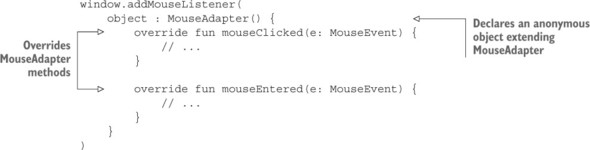
\includegraphics[width=11cm]{object-expression}
  \caption{\emph{Object Expression}. Fuente \cite{kotlin-in-action}}
  \label{fig:object-expression}
\end{figure} 

\subsection{Declaraciones, manejo del alcance de los identificadores} \label{sec:declaraciones}

\subsubsection{Declaración de tipos}
Nuevos tipos son introducidos en Kotlin a través de clases, \texttt{Data Classes}, \texttt{Enum Classes}, interfaces y objetos.

\paragraph{Declaración de una clase}
\begin{verbatim}
    class Invoice {
    }
    // Clase con constructor primario
    class User(_nickname: String) {
        val nickname = _nickname
    }
    // 
    val invoice = Invoice()
    val user = User("Luigi")    
\end{verbatim}

\paragraph{Data Classes} Clases cuyo propósito principal es contener datos. En una clase de este tipo, algunas funcionalidades estándar y funciones de utilidad a menudo se derivan mecánicamente de los datos.
\begin{verbatim}
    data class User(val name: String, val age: Int)
    val admin = User("John", 40)
\end{verbatim}

El compilador automáticamente deriva los siguientes miembros para todas las propiedades declaradas en el constructor primario: \texttt{equals(), hashCode()}, \texttt{toString()}, \texttt{copy()}. Para asegurar la consistencia y significado del código generado, las \emph{data classes} tiene que tener los siguietes requisitos:
\begin{itemize}
    \item El constructor primario necesita tener al menos un parámetro
    \item Todos los parámetros del constructor primario necesitan estar marcados con \texttt{val} o \texttt{var}
    \item \emph{Data classes} no pueden ser abstractas, internas o selladas (\emph{sealed}).
\end{itemize}

\paragraph{Enum Classes}
\begin{verbatim}
    enum class Color {
        RED, ORANGE, YELLOW, GREEN, BLUE, INDIGO, VIOLET
    }
    //
    val primaryColor = Color.GREEN
\end{verbatim}

\paragraph{Interfaces}
Interfaces en Kotlin son similares a las de Java8: pueden contener definiciones de métodos abstractos así como implementaciones de métodos no abstractos (similar a los métodos \emph{default} de Java8), pero no pueden contener ningún estado.
\begin{verbatim}
    interface Clickable {
        fun click()
    }
    
    class Button : Clickable {
        override fun click() = println("I was clicked")
    }
    val submitBtn : Clickable = Button()
    submitBtn.click() 
    
    // Interfaz con implementaciones
    interface Focusable {
        fun setFocus(b: Boolean) = 
            println("I \${if (b) "got" else "lost"} focus.")
            
        fun showOff() = println("I'm focusable!")            
    }
\end{verbatim}


\paragraph{Objetos}



%En la sección \ref{sec:variables-almacenamiento}, se introdujo las palabras reservadas \texttt{val} y \texttt{var} para declarar una variable. Las siguientes declaraciones enlazan un identificador (a la izquierda) con un nuevo tipo.
%
%\begin{verbatim}
%    val myNumber = 40          // Int
%    val name = "Charles"       // String
%    val isActive = true        // Boolean
%    val employee = Employee()  // Clase, Data Class, Object
%\end{verbatim}


\subsubsection{Declaración de constantes}
Las propiedades cuyo valor se conoce en tiempo de compilación se pueden marcar como constantes de tiempo de compilación (\emph{compile time constants}) utilizando el modificador \texttt{const}. Estas propiedades necesitan tener los siguientes requerimientos:
\begin{itemize}
    \item Tiene que ser un miembro de primer niven en un \emph{object}
    \item Inicializado con un valor de tipo \texttt{String} o un valor primitivo
    \item Sin un \emph{getter} personalizado
\end{itemize}

\begin{verbatim}
    const val COUNTRY: String = "Costa Rica"
\end{verbatim}

\subsubsection{Declaración de variables}
Véase sección \ref{sec:variables-almacenamiento}.

\subsubsection{Declaración de funciones y procedimientos}
\begin{itemize}
    \item La palabra reservada \texttt{fun} se utiliza para declarar una función. 
    \item El tipo de parámetro se escribe luego de su nombre. Esto aplica también para declaraciones.
    \item La función se puede declarar en cualquier parte del archivo, no se necesita poner dentro dentro de una clase.
\end{itemize}

\begin{figure}[h!]
  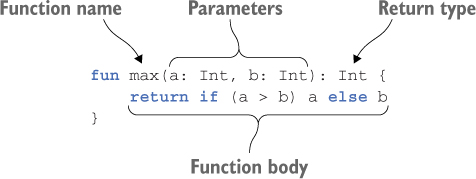
\includegraphics[width=8.7cm]{function}
  \caption{Declaracion de una función en Kotlin. Fuente \cite{kotlin-in-action}}
  \label{fig:kotlin-function-declaration}
\end{figure} 

La declaración de la función inicia con la palabra clave \texttt{fun}, seguida del nombre de la función: \texttt{max} en en caso del ejemplo de la figura \ref{fig:kotlin-function-declaration}. El tipo de retorno viene luego de la lista de parámetros, separado por dos puntos. Nótese que en Kotlin, \texttt{if} es una expresión con un valor como resultado. Es similar como al operador ternario de Java: 
\begin{verbatim}
    (a > b) ? a : b
\end{verbatim}

\subsubsection{Manejo del alcance de los identificadores}
Kotlin no introduce ningún cambio en el manejo del alcance de los identificadores en comparación con Java. Los identificadores ``viven'' dentro del ámbito en el que fueron declaradas (clases, funciones, bloques).

\subsection{Estructuras de control}

\paragraph{Expresión \texttt{if}}
Uso tradicional
\begin{verbatim}
    var max = a
    if (a < b) max = b
\end{verbatim}

\paragraph{Utilizando \texttt{else}}
\begin{verbatim}
    var max : Int
    if (a > b) {
        max = a
    } else {
        max = b
    }
\end{verbatim}

\paragraph{Como expresión}
\begin{verbatim}
    val max = if(a > b) a else b
\end{verbatim}




\subsubsection{Expresión \texttt{when}}
reemplaza al operador \emph{switch} de lenguajes basados en \texttt{C}. Evalua el argumento contra todos los caso de manera secuencial hasta que se cumpla una de las condiciones. El caso \texttt{else} se evalua si ninguno de los otros casos se pudo satisfacer. Puede utilizar expresiones arbitrarias(no solo constantes) y también se puede evaluar si un valor se encuentra dentro de un rango.
\begin{verbatim}
    when (x) {
        1          -> print("x == 1")
        2          -> print("x == 2")
        3, 4       -> print("x == 3 or x == 4")
        in 5..10   -> print("x is between 5 and 10")
        !in 20..30 -> print("x is outside the range")
        else -> {
            print("none of the above")
        }
    }
\end{verbatim}

\subsubsection{Ciclos \texttt{for}} 
Tiene una forma equivalente al ciclo \texttt{for-each} de Java.
\begin{verbatim}
    for (item: Int in ints) {
        print(item)
    }
\end{verbatim}

Se puede iterar sobre un rango de números:
\begin{verbatim}
    for (i in 1..3) {
        println(i)
    }
    for (i in 6 downTo 0 step 2) {
        println(i)
    }
\end{verbatim}


\subsubsection{Ciclos \texttt{while}}
Tanto el ciclo \texttt{while} como el \texttt{do..while} trabajan de la misma forma que en Java:
\begin{verbatim}
    while (x > 0) {
        x--
    }
    
    do {
        val y = retrieveData()
    } while (y != null) // y es visible aquí
\end{verbatim}

\subsection{Secuenciadores}
% manejo de escapes, excepciones, continuaciones
Kotlin tiene tres expresiones para saltos/continuaciones:
\begin{itemize}
    \item \texttt{return}: retorna de la función más cercana
    \item \texttt{break}: termina un ciclo 
    \item \texttt{continue}: continua con el siguiente paso de un ciclo 
\end{itemize}

\paragraph{\texttt{break} y \texttt{continue} con etiquetas}
Cualquier expresión en Kotlin puede ser etiquetada. Las etiquetas tienen un identificador seguido del signo \texttt{@}. Para etiquetar una expresión, se punta una etiqueta en frente de ella
\begin{verbatim}
    loop@ for (i in 1..100) {
        //...
    }
\end{verbatim}

Se puede marcar un \texttt{break} o un \texttt{continue} con una etiqueta:
\begin{verbatim}
    loop@ for (i in 1..100) {
        for (j in 1..100) {
            if (...) break@loop
        }
    }
\end{verbatim}
Un \texttt{break} marcado con una etiqueta salta al punto de ejecución justo después del ciclo que fue marcado con esa etiqueta. Un \texttt{continue} prosigue con la próxima iteración del ciclo.

\paragraph{Excepciones}
Todas las excepciones en Kotlin son descendientes de la clase \texttt{Throwable}. Todas las excepciones tienen un mensaje, un \emph{stack trace} y una causa (opcional). Para lanzar una excepción se usa la expresión \texttt{throw}
\begin{verbatim}
    throw MyException("Hi There!")
\end{verbatim}

Para atrapar una excepción, se usa la expresión \texttt{try}:
\begin{verbatim}
    try {
        // algún código
    } catch (e: SomeException) {
        // código manejador de excepción
    } finally {
        // bloque finalizador opcional
    }
\end{verbatim}
Pueden haber uno o varios bloques \texttt{catch}. Los bloques \texttt{finally} pueden ser omitidos. 

\subsection{Mecanismos de abstracción}
%% Esta sección podria ser reemplazada por otras en donde se habla sobre clases, subclases, herencia, tipos abstractos, encapsulacimiento

\subsection{Mecanismos de modularización}
Java organiza todas las clases en paquetes. Kotlin también tiene el concepto de paquetes. Cada archivo Kotlin puede tener una declaración de \texttt{package} al inicio y, todas las demás declaraciones (clases, funciones y propiedades) definidas en el archivo serán colocados bajo ese paquete. Las declaraciones definidas en otros archivos puede ser usados directamente si ellos están en el mismo paquete. Si se encuentran en diferentes paquetes necesitan ser importados. Tal y como en Java las declaraciones de importación se colocan al inicio del archivo por medio de la palabra reservada \texttt{import}. En la figura \ref{fig:import-1} se muestra un ejemplo de una declaración de \texttt{package} e \texttt{import} en un archivo.

\begin{figure}[h!]
  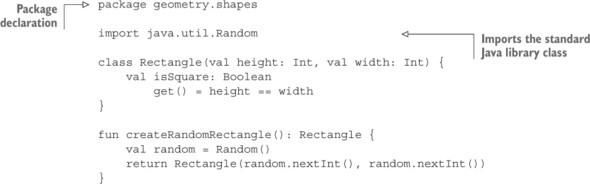
\includegraphics[width=12cm]{import-1}
  \caption{Declaracion de una clase y una función en un paquete. Fuente \cite{kotlin-in-action}}
  \label{fig:import-1}
\end{figure}  

Kotlin no hace distinción entre importar clases y funciones, y esto permita importar cualquier clase de declaración usando la declaración \texttt{import}.

\begin{figure}[h!]
  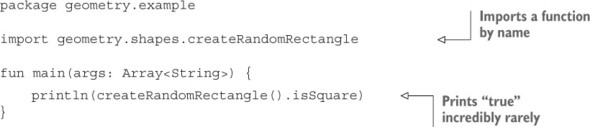
\includegraphics[width=12cm]{import-2}
  \caption{Importando una función desde otro paquete. Fuente \cite{kotlin-in-action}}
  \label{fig:import-2}
\end{figure}

También se puede importar todas las declaraciones de un paquete en particular poniendo \texttt{.*} luego del nombre del paquete. Este \emph{star import} hace visible no solamente las clases definidas del paquete sino también funciones y propiedades. Si en la figura \ref{fig:import-2} se escribiera \texttt{import geometry.shapes.*} en lugar de la importación explícita, el código continuaría siento correcto.

En Kotlin, se pueden poner varias clases en el mismo archivo y se escoger cualquier nombre para ese archivo. Kotlin no impone ninguna restricción en cómo se disponen los archivos en el disco. Se puede usera cualquier estructura de directorios para organizar los archivos. Sin embargo, en la mayoría de los caso es una buena práctica seguir la estructura de directorios de Java para organizar los archivos. Esta estructura se hace particularmente importante en proyectos en donde se combina código Java y Kotlin porque ayuda a migrar el código gradualmente.

\subsection{Soporte a concurrencia, paralelismo, distribución}
Al ser 100\% interoperable con Java, en Kotlin se pueden utilizar todas las librerías (\emph{Futures}, \emph{CompletableFutures}, \emph{Reactive Extensions}) para concurrencia, paralelismo y programación asincrónica en general que son utilizadas en Java.

\subsubsection{Corutinas (\emph{Coroutines})}
A partir de la versión 1.1 de Kotlin se introdujo el concepto de Corutina que proporciona una forma de evitar bloquear un hilo(\emph{thread}) y reemplazarlo con una operación más económica y de mayor control: la \emph{suspensión} de una corutina.

Básicamente, las corutinas son cómputos que pueden ser \emph{suspendidos} sin bloquear un hilo. El bloqueo de un hilo es usualmente una operación cara en términos de CPU y memoria, especialmente bajo grandes cargas de trabajo, porque solamente un número relativamente pequeño de hilos puede ser mantenido, por lo que bloquear uno de ellos lleva a que se retrase un trabajo importante.

Por otro lado, la suspensión de una corutina es casi gratis. No hay cambios de contexto o cualquier otro tipo de involucramiento del sistema operativo es requerido. Aparte de esto, la suspensión puede ser contralada por el código del usuario y de esta forma decidir qué pasa con la misma y de esta forma optimizar, interceptar o capturar una excepción de acuerdo al escenario dado.

Otra diferencia es que las corutinas no pueden ser suspendidas a partir de cualquier instrucción, sino solmanete con los llamados puntos de suspensión(\emph{suspension points}), que son llamados a funciones con anotadas de manera especial(\texttt{suspend}).

\paragraph{Suspendiendo funciones} una suspensión pasa cuando se llamada a una función marcada con la palabra reservada \texttt{suspend}:
\begin{verbatim}
    suspend fun doSomething(foo: Foo): Bar {
        ...
    }
\end{verbatim}
Estas funciones son llamadas \emph{suspending functions} porque las llamadas a ellas pueden suspender una corutina. Las \emph{suspending functions} pueden tomar parámetros y retornar valores de la misma forma que las funciones normales, pero solamente pueden ser llamadas desde corutinas y otras \emph{suspending functions}.

De hecho para iniciar una corutina, debe de haber al menos una \emph{suspending function}, y es usualmente una función lambda. El siguiente es un ejemplo simplificado de la función \texttt{async}\footnote{De la librería kotlinx.coroutines}.
\begin{verbatim}
    fun <T> async(block: suspend() -> T)
\end{verbatim}
En el ejemplo, \texttt{async} es una función normal pero el parámetro \texttt{block} es de tipo función con la palabra reservada \texttt{suspend}: \texttt{suspend() -> T}. De esta forma, cuando se pasa una función lambda a \texttt{async}, es una \emph{suspending lambda}, y se puede invocar una \emph{suspending function} desde ahi.

\paragraph{\texttt{RxKotlin}\cite{rxkotlin}} La programación reactiva es un paradigma de programación asincrónica que gira en torno a flujos de datos \emph{streams} y propagación de cambios. Los programas que propagan todos los cambios que afectaron sus datos o sus flujos de datos (a usuarios finales, componentes u otro programa relacionado) son llamados programas reactivos.

\texttt{RxKotlin} es una implementación específica de programación reactiva para Kotlin, que está influenciada en programación funcional. Favorece composición de funciones, evita el manejo de estados globales y efectos secundarios. Se basa en el patrón observador $\rightarrow$ productor/consumidor, con muchos operadores que permiten componer, calendarizar(\emph{scheduling}), transformar y gestionar errores.
 

\subsection{Sistemas de tipos} \label{sec:tipos}
Como se señaló en la sección \ref{sec:declaraciones}, nuevos tipos son introducidos en Kotlin a través de clases, Data Classes, Enum Classes, interfaces y objetos. 

\paragraph{Modificadores de acceso para clases:} \texttt{open}, \texttt{final} y \texttt{abstract}. 
\begin{itemize}
    \item \texttt{final}: \underline{No} puede ser sobre escrita. Utilizada por defecto para los miembros de clase
    \item \texttt{open}: Puede ser sobreescrita. Tiene que se especificada explícitamente
    \item \texttt{abstract}: \underline{Debe} ser sobre escrita. Puede ser utilizada solamente en clases abstractas, los miembros abstractos no pueden tener una implementación
    \item \texttt{override}: sobre escribe un miembro de una super clase o interfaz. El miembro sobreescrito está abierto por defecto, sino está marcado como \texttt{final}. 
\end{itemize}

\paragraph{Modificadores de visibilidad:} 
\begin{itemize}
    \item \texttt{public} (por defecto). Visible en todas partes
    \item \texttt{internal}. Visible en un módulo
    \item \texttt{protected}. Visible en subclases
    \item \texttt{private}. Visible en una clase
\end{itemize}

\subsubsection{Herencia}
Todas las clases en Kotlin tienen una superclase \texttt{Any} en común, esta es la superclase por defecto para una clase sin ningún super tipo declarado:
\begin{verbatim}
    class Example // Implícitamente hereda de Any
\end{verbatim}

Para declarar un super tipo de forma explícita, se pone el tipo después de dos puntos en el encabezado de la clase:
\begin{verbatim}
    open class Base(p: Int)
    
    class Derived(p: Int) : Base(p)
\end{verbatim}
 
Si la clase derivada tiene un constructor primario, la clase base puede (y debe) ser inicializada de una vez, utilizando los parámetros del constructor primario. Si la clase no tiene un constructor primario, entonces cada constructor secundario tiene que inicializar el tipo base utilizando la palabra reservada \texttt{super}, o bien, delegar a que otro constructor lo haga. 

\begin{verbatim}
    class MyView : View {
        constructor(ctx: Context) : super(ctx)
        
        constructor(ctx: Context, attrs: AttributeSet) : super(ctx, attrs)
    }
\end{verbatim}

\subsubsection{Sobreescritura de Métodos}
Kotlin requiere anotaciones explícitas para miembros que pueden ser sobreescritos(\texttt{open}) y para las sobreescrituras como tal:
\begin{verbatim}
    open class Base {
        open fun v() {}
        fun nv() {}
    }
    class Derived() : Base() {
        override fun v() {}
    }
\end{verbatim}

La palabra reservada \texttt{override} es requerida en \texttt{Derived.v()}. Si no hay una anotación \texttt{open} en una función, como en \texttt{Base.nv()}, la declaración de un métodos con la misma firma en una subclase sería ilegal.

\subsubsection{Extensiones}
De manera similar a \texttt{C\#}, Kotlin proporciona la habilidad de extender una clase con nueva funcionalidad sin tener que heredar de la clase o usar algún tipo de patrón de diseño como el patrón decorador\footnote{Patrón Decorador: \url{https://en.wikipedia.org/wiki/Decorator_pattern}}. Esto se realiza por medio de una declaración especial llamada extensión. Kotlin soporta funciones y de propiedades extendidas (\emph{extension functions} y \emph{property extension} ).

\paragraph{Extension functions} Para su declaración se necesita añadir el tipo que va a ser extendido como prefijo del nombre. El siguiente código añade la función \texttt{swap} a \emph{MutableList<Int>}:
\begin{verbatim}
    fun MuchableList<Int>.swap(index1: Int, index2: Int) {
        val tmp = this[index1] //'this' corresponde a la lista
        this[index1] = this[index2]
        this[index2] = tmp
    }
   // Uso
   val l = mutableListOf(1, 2, 3)
   l.swap(0,2) 
\end{verbatim}
La palabra reservada \texttt{this} dentro de un \emph{extension function} corresponde al objecto que es pasado antes del punto.

\paragraph{Las extensiones son resueltas estáticamente} Las extensiones no modifican las clases con su extención. Cuando se define una extensión, no se insertan nuevos miembros en la clase sino que se hace que las funciones puedan ser invocadas por medio de la notación basada en punto (\emph{dot notation}) en las variables de este tipo.

\paragraph{Extension properties} 
\begin{verbatim}
    val <T> List<T>.lastIndex: Int
        get() = size - 1
\end{verbatim}


\subsection{Genericidad}
Tal y como el Java, las clases en Kotlin pueden tener tipos parametrizados:
\begin{verbatim}
    class Box<T>(t: T) {
        var value = t
    }
    //Uso
    val box: Box<Int> = Box<Int>(1)
    val box: Box(1) // 1 es de tipo Int, asi que se puede hacer inferir el tipo
\end{verbatim}

\subsubsection{Varianza}
Una de las partes más difíciles de los tipo de Java son los tipos \emph{wildcard}\footnote{\url{http://www.angelikalanger.com/GenericsFAQ/JavaGenericsFAQ.html}}. Kotlin no tiene ninguno de estos.

\paragraph{Declaration-site variance vs. Java wildcards} 
Supóngase que se tiene una interfaz \texttt{Source<T>} que no tiene ningún método que tome \texttt{T} como parámetro, solamente tiene métodos que retornan \texttt{T}:
\begin{verbatim}
    //Java
    interface Source<T> {
     T nextT();
    }
\end{verbatim}
Podría ser seguro almacenar una reference a una instancia de \texttt{Source<String>} en una variable de tipo \texttt{Source<Object>}, pero Java no sabe de esto y lo prohibe:
\begin{verbatim}
    //Java
    void demo(Source<String> strs) {
        Source<Object> objects = strs // NO se permite en Java
    }
\end{verbatim}
Para arreglar esto, se tiene que declarar \texttt{objects} de tipo \texttt{Source<? extends Object>}. En Kotlin, existe una forma de explicar esto al compilador. Se le llama \emph{declaration-site variance}: se puede another el tipo parametrizado \texttt{T} de \texttt{Source} para asegurarse de que solo se devuelve(produce) a partir de miembros de \texttt{Source<T>}. Para hacer esto se proporciona el modificador \texttt{out}.
\begin{verbatim}
    interface Source<out T> {
        fun nextT() : T
    }
    
    fun demo(strs : Source<String>) {
        val objects : Source<Any> = strs // Esto está bien porque T es un out-parameter
    } 
\end{verbatim}
 
Al modificador \texttt{out} se le llama anotación de varianza y, debido a que es proporcionado en la declaración del tipo parametrizado, se llama \emph{declaration-site variance}. 
Ademas de \texttt{out}, Kotlin provee una anotación complementaria de varianza: \texttt{in}, hace que un tipo parametrizado solo puede ser consumido pero nunca producido.
\begin{verbatim}
    interface Comparable<in T> {
        operator fun compareTo(other: T) : Int
    }    
    
    fun demo(x: Comparable<Number>){
        x.compareTo(1.0) // 1.0 es de tipo Double, que es un subtipo de Number
        // Por lo tanto, se puede asignar x a una variable de tipo Comparable<Double>
        val y : Comparable<Double> = x // OK!
    }
\end{verbatim}

\paragraph{Star projections}
Existen situaciones en donde no se tiene conocimiento del tipo específico del tipo del valor. Supóngase que solamente se desea imprimir todos los elementos de un arreglo y que no importa el tipo de los elemento en ese arreglo. Para esto se puede utlizar una \emph{star projection}:
\begin{verbatim}
    fun printArray(array: Array<*>) {
        array.forEach { println(it) }
    }
    // Uso
    val array = arrayOf(1, 2, 3)
    printArray(array)
\end{verbatim}

\subsubsection{Funciones genéricas}
No solamente las clases pueden tener tipos parametrizados, las funciones también pueden tenerlo. Los tipos parametrizados se colocan antes del nombre de la función. En la figura \ref{fig:kotlin-generic-function-declaration} se puede ver un ejemplo.
\begin{figure}[h!]
  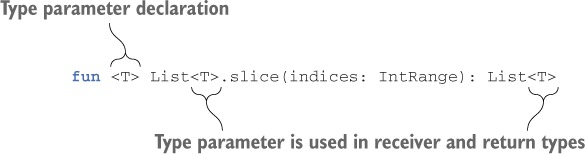
\includegraphics[width=8.7cm]{generic-function}
  \caption{Declaracion de una función genérica en Kotlin. Fuente \cite{kotlin-in-action}}
  \label{fig:kotlin-generic-function-declaration}
\end{figure} 
\begin{verbatim}
    //Uso
    val letters = ('a'..'z').toList()
    println(letters.slice<Char>(0..2))
    -> [a, b, b]
    println(letters.slice(10..13))
    -> [k, l, m, n]
\end{verbatim}



\subsection{Soporte a paradigmas}
%% objetos, funciones, datos, etc
Los dos grandes paradigmas soportados por Kotlin son: programación orientada a objetos y programación funcional. Características de programación orientada a objetos se han señalado en secciones anteriores y se ha visto como las clases son consideradas como ``ciudadanos de primera clase'' para introducir nuevos tipos y modelado de programas a través de interfaces, herencia, tipos parametrizados, entre otros.

Además de las clases, las funciones son también consideradas de primera clase en Kotlin, lo que significa que puede ser almacenadas en variables y estructuras de datos, pasadas como argumentos y retornadas desde otra funcion de orden superior (\emph{high-order function}: una función que toma funciones como parámetro o retorna una función). Aparte de esto, Kotlin ofrece un amplio conjunto de funcionalidades para programación funcional dentro de las que destacan las expresiones lambda, \emph{data classes} e interfaces de programación para trabajar con objetos y colecciones siguiendo un estilo funcional.

Kotlin permite que se pueda programar de forma funcional pero no obliga a esto. Cuando se escribe código en Kotlin se puede combinar ambos enfoques y usar las herramientas que sean más apropiadas para el problema que se resuelve.

Por último, Kotlin también puede ser utlizado como un lenguaje de \emph{scripting}. Se puede utilizar las utilidad \texttt{kotlinc} como un REPL(\emph{Read-Eval-Print Loop}) o bien para ejecutar archivos de \emph{scripting} de Kotlin \texttt{.kts}
\begin{verbatim}
    > kotlinc // Inicia el REPL
    > kotlinc -script sample.kts // Ejecuta el código Kotlin dentro de sample.kts
\end{verbatim}

\subsection{Soporte a ``programación en grande''}
Kotlin ha ganado mucha popularidad en los últimos 3 años. Esto ha sido motivado principalmente por su interoperatibilidad con Java además del soporte de primera clase de que le han brindado proyectos tales como Android y \emph{Spring Framework}, dos de los más populares dentro de la comunidad de desarrolladores de Java.

Otra de las ventajas que tiene Kotlin tanto como lenguaje y plataforma es su versatilidad. Con Kotlin se puede programar aplicaciones \emph{backend} utilizando proyectos como \emph{Spring}\footnote{\url{https://spring.io/}}, Vert.x\footnote{\url{http://vertx.io/}} y Ktor\footnote{\url{https://github.com/kotlin/ktor}}. Se pueden programar aplicaciones móviles con Android. Se puede transpilar código Kotlin a JavaScript para hacer aplicaciones del lado del cliente y también para hacer aplicaciones del lado del servidor utilizando NodeJS. Por último el proyecto Kotlin/Native\footnote{\url{https://github.com/JetBrains/kotlin-native/}} es una tecnología para compilar Kotlin a binarios nativos que pueden correr sin necesidad de una máquina virtual. Este proyecto está pensado principalmente para permitir la compilación en plataformas en donde las máquinas virtuales no se pueden utilizar como en en sistemas embebidos, o cuando el desarrollador necesita producir programas que no requieran de ambientes de ejecución adicionales.

\paragraph{¿Quiénes usan Kotlin?} Se ha reportado que compañías tales como Google, Amazon, Netflix, Pinterest, Uber, Foursquare, Trello, Capital One, Coursera, Basecamp, Corda, JetBrains, Pivotal, Evernote, entre otros usan Kotlin para el desarrollo de sus aplicaciones.

\subsection{Pecularidades}
%% expresiones regulares, concurrencia, concordancia de patrones, retroceso

\section{Ejemplos}

\section{Análisis y conclusiones}

\bibliographystyle{ACM-Reference-Format}
\begin{thebibliography}{9}

\bibitem{kotlin-in-action} Dmitry Jemerov, Svetlana Isakova. \emph{Kotlin in Action}. Manning Publications Company. 2017. ISBN 9781617293290

\bibitem{krill} Krill, Paul \emph{JetBrains readies JVM language Kotlin}. infoworld.com. InfoWorld. 2011. Obtenido el 11 de Abril del 2018 de \url{https://www.infoworld.com/article/2622405/java/jetbrains-readies-jvm-based-language.html}.

\bibitem{kotlin-v1} Kotlin Blog. \emph{Kotlin 1.0 Released: Pragmatic Language for JVM and Android}". Febrero, 2015. Obtenido el 11 de Abril del 2018 de \url{https://blog.jetbrains.com/kotlin/2016/02/kotlin-1-0-released-pragmatic-language-for-jvm-and-android/}

\bibitem{kotlin-in-android} Kotlin Blog. \emph{Kotlin on Android. Now official}. Mayo, 2017. Obtenido el 11 de Abril del 2018 de \url{https://blog.jetbrains.com/kotlin/2017/05/kotlin-on-android-now-official/}.

\bibitem{kotlin-v12} Kotlin Blog. \emph{Kotlin 1.2 Released: Sharing Code between Platforms}. Noviembre, 2017. Obtenido el 11 de Abril del 2018 de \url{https://blog.jetbrains.com/kotlin/2017/11/kotlin-1-2-released/}.

\bibitem{rxkotlin} Rivu Chakrabory. \emph{Reactive Programming in Kotlin}. Packt Publishing. Diciembre 2017. IBSN: 9781788473026

\bibitem{kotlin-ref} Kotlin. \emph{Kotlin Reference}. \url{https://kotlinlang.org/docs/reference}

\end{thebibliography}



%\newpage
%\section{Performance evaluation of component-based software systems: A survey\cite{performance-model-survey}}
%
%Durante los últimos diez años, los investigadores han propuesto muchos enfoques para evaluar el rendimiento (tiempos de respuesta, \emph{throughput}, utlización de recursos) de sistemas de software basados en componentes. Estos enfoques lidian con predicción de rendimiento y medición del rendimiento. Los primeros analizan el rendimiento esperado de un diseño de software basado en componentes para evitar problemas de rendimiento en la implementación del sistema, lo que podría llevar a costos substanciales para rediseñar la arquitectura. Los otros analizan el rendimiento observable de sistemas de software basados en componentes implementados para entender sus propiedades, determinar su capacidad máxima, identificar componentes críticos y para remover cuellos de botella.
%
%\paragraph{\textbf{Métodos de evaluación de rendimiento}}
%Los enfoques se agruparon en dos grandes grupos: enfoques principales que proporcionan procesos de evaluación de rendimiento completo y enfoques suplementarios que se centran en aspectos específicos como medición de componentes individuales o modelaje de las propiedades de rendimiento de los conectores de un componente.
%
%\paragraph{Enfoques principales} 
%\begin{itemize}
%    \item Enfoques de predicción basados en UML:
%    \begin{itemize}
%        \item CB-SPE - \emph {The Component-Based Software Performance Engineering}
%    \end{itemize}
%    \item Enfoques de predicción basados en meta-modelos propietarios
%    \begin{itemize}
%        \item CBML - \emph{The Component-Based Modelling Language}
%        \item PECT - \emph{The Prediction Enabled Component Technology}
%        \item COMQUAD - \emph{Components with Quantitative properties and Adaptivity}
%        \item KLAPPER
%        \item ROBOCOP
%        \item PALLADIO 
%    \end{itemize}
%    \item Enfoques de predicción centrados en \emph{middleware}
%    \begin{itemize}
%        \item NICTA
%    \end{itemize}
%    \item Enfoques basados en especificaciones formales
%    \begin{itemize}
%        \item RESOLVE
%        \item HAMLET
%    \end{itemize}
%    \item Enfoques de monitoreo para sistemas implementados
%    \begin{itemize}
%        \item COMPAS
%        \item TESTEJB
%        \item AQUA
%        \item PAD
%    \end{itemize}
%\end{itemize}
%
%\paragraph{Enfoques Suplementarios}
%\begin{itemize}
%    \item Enfoques de monitoreo para componentes implementados
%    \begin{itemize}
%        \item RelCAM
%        \item COMAERA
%        \item BYCOUNTER
%    \end{itemize}
%    \item{Enfoques de predicción para conectores de componentes}
%    \begin{itemize}
%        \item Verdickt
%        \item Grassi
%        \item Becker
%        \item Happe
%    \end{itemize}
%\end{itemize}
% 
%
%
%\newpage
%\section{The Palladio component model for model-driven performance prediction\cite{palladio-seminal}}
%
%El el desarrollo de software basado en componentes (CBSE, por sus siglas en inglés) la idea central es construir sistemas de software complejo uniendo componentes básicos. El objetivo inicial de CBSE fue incremetar el nivel de reutilización. Sin embargo, estructuras compuestas también pueden aumentar el nivel de predictibilidad del sistema durante etapas tempranas de desarrollo, esto porque modelos certificados de componentes individuales pueden ser compuestos, permitiendo a los arquitectos de software razonar sobre la estructura compuesta. Esto es importante para las propiedades funcionales, pero también para las propiedades extra funcionales como rendimiento y confiabilidad. 
%
%Los métodos para predicción de rendimiento y confiabilidad de sistemas de software en general son limitados y raramente usados en la industria. Este reto es aún mayor en CBSE debido a que varios roles independientes están involucrados en la creación del sistema. Muchos métodos existentes para predicción de CBSE requieren que los arquitectos de software modelen el sistema basados en especificaciones de un solo componente. Luego se asume que el arquitecto proporcionará información faltante. Otros enfoques dejan de lado factores que afectan el rendimiento percibido de un componente de software tal y como la influencia de servicios externos, cambio de recursos de su ambiente o diferentes parámetros de entrada. Sin embargo, para predicciones precisas, todas estas dependencias tiene que hacerse explícitas en la especificación del componente.
%
%Con \emph{Palladio\footnote{Toma su nombre del arquitecto renacentista Andrea Palladio (1508 - 1580) quien de cierta forma, intentó predecir el impacto estético de sus construcciones por adelantado.} Component Model} (PCM) un meta-modelo provee la especificación de información relevante del rendimiento de una arquitectura basada en componentes. El diseño y análisis de estos meta-modelos son los primeros que explícitamente incluyen todos los factores que influencian el rendimiento de un componente de software como lo son: la implementación, rendimiento de servicios externos, rendimiento del ambiente de ejecución y el perfil de uso. El modelo es diseñado con especial énfasis en la predicción de atributos de calidad de servicio como el rendimiento y la confiabilidad.
%
%En el proceso de CBSE(figura \ref{fig:palladio-cbse}) los autores distinguen cuatro tipos de roles involucrados en la producción de artefactos de un sistema de software: \emph{desarrolladores de componentes} especifican e implementan los componentes, \emph{arquitectos de software} ensamblan componentes para construir aplicaciones, \emph{system deployers} modela los recursos del ambiente y luego su asignación, \emph{expertos del dominio de negocio} que están familiarizados con los usuarios del sistema y proporcionan modelos de su uso. El modelo completo del sistema puede ser derivado a partir de modelos parciales especificados por cada uno de los roles para que luego las propiedades extra funcionales puedan ser predecidas.
%
%%\begin{figure}[h!]
%%  \includegraphics[width=8.7cm]{palladio-cbse-process}
%%  \caption{Proceso CBSE propuesto por PCM}
%%  \label{fig:palladio-cbse}
%%\end{figure} 
%
%
%\newpage
%\section{Performance-oriented DevOps: a research agenda\cite{performance-devops}}
%DevOps es una tendencia hacia una estrecha integración entre equipos desarrollo y operaciones. La necesidad de tal integración es orientada por el requerimiento de adaptar aplicaciones empresariales a los cambios del ambiente del negocio continuamente. El rendimiento describe las propiedades del sistema con respecto a su ejecución y uso de recursos. Métricas comunes son tiempo de respuesta, \emph{throughput} y la utilización de los recursos. Los objetivos de rendimiento para aplicaciones empresariales son típicamente definidos al establecer cotas superiores/inferiores para estas métricas y transacciones de negocio específicas.
%
%\subsection{Actividades de administración del rendimiento}
%\subsubsection{Evaluación del rendimiento basado en modelos}
%\begin{itemize}
%    \item La representación de la memoria principal y del recolector de basura aún no están explícitamente integrados ni considerados en los modelos de rendimiento
%    \item La selección de técnicas apropiadas de solución requiere de mucha experiencia
%\end{itemize}
%
%\subsubsection{Extracción de modelos de rendimiento y de cargas de trabajo}
%\begin{itemize}
%    \item La precisión de los modelos puede llegar a expirar si no son actualizados cuando hay cambios. Mecanismos de detección son requeridos para aprender cuando los modelos son antiguos y hay que actualizarlos.
%    \item La extracción de capacidades de rendimiento se basa en una combinación de software y los recursos de hardware en los que se implementa. Este enfoque combinado es compatible con la precisión de la predicción, pero está menos calificado con respecto a la portabilidad de los conocimientos a otras plataformas. Una dirección de investigación futura podría ser extraer modelos separados (por ejemplo, \emph{middleware} y modelos de aplicación separados). 
%\end{itemize}
%
%
%
%\subsection{Ingeniería de rendimiento de software durante el desarrollo}
%
%\subsubsection{Modelos de rendimiento durante etapas diseño }
%\begin{itemize}
%    \item Los retos de utilizar modelos de rendimiento en etapas tempranas de desarrollo es que usualmente es difícil validar la precisión de los modelos hasta que un sistema en ejecución exista. Las predicciones de rendimiento basadas en suposiciones, entrevistas y pruebas previas pueden ser también imprecisas y por tanto las decisiones que se hagan a partir de estas predicciones.
%\end{itemize}
%
%
%\paragraph{Sobre este reporte} Este es un reporte extenso que da a conocer retos y oportunidades en investigación sobre DevOps y rendimiento. En este resumen se incluyeron varios de los puntos más relevantes concernientes a modelaje del rendimiento. 
%
%
%
%
%
%\newpage
%\section{Performance Engineering for Microservices: Research Challenges and Directions\cite{microservices-challenges}}
%Los microservicios complementan enfoques como DevOps y entrega continua(CD por sus siglas en inglés) en relación en términos de arquitectura de software. Junto con este estilo de arquitectura, otras tecnologías importantes para \emph{deployment} como, virtualización basada en contenedores y soluciones de orquestación de contenedores han emergido. Estas tecnologías permiten explotar plataformas en la nube, proporcionando altos niveles de escalabilidad, disponibilidad y portabilidad para microservicios. A pesar del hecho de que es una necesidad inherente contar con escalabilidad y elasticidad, la ingeniería de rendimiento para microservicios hasta ahora ha tenido poca atención por parte de las comunidades tanto de microservicios como de comunidades de investigación de ingeniería de rendimiento. Un gran cuepro de conocimiento y buenas prácticas para ingeniería de rendimiento para desarrollo tradicional de software y arquitecturas está disponible. Sin embargo, sus aplicaciones en DevOps imponen tanto retos como oportunidades.
%
%\subsection{Retos de investigación}
%
%\subsubsection{Pruebas de rendimiento}
%\begin{itemize}
%    \item Reemplazar y compensar pruebas extensivas de integración y de sistema por un control detallado de los entornos de producción
%    \item Alinear las pruebas de rendimiento y pruebas de regresión de rendimiento con prácticas de entrega continua, por ejemplo, acelerar las estas de pruebas correspondientes.
%    \item Selección dinámica y semi automática de pruebas de rendimiento
%\end{itemize}
%
%\subsubsection{Monitoreo}
%\begin{itemize}
%    \item Instrumentación para monitoreo distribuido arquitecturas microservicios políglotas 
%    \item Métricas adicionales para monitorear microservicios
%    \item Técnicas de detección precisa de anomalías en arquitecturas de microservicios
%\end{itemize}
%
%
%\subsubsection{Modelado del rendimiento}
%De momento no existen enfoques para modelado del rendimiento de microservicios 
%\begin{itemize}
%    \item Adoptar modelos de rendimiento para casos de uso como planeamiento de capacidad, confiabilidad y resiliencia
%    \item Buscar abstracciones de modelado apropiadas 
%    \item Extracción automática de modelos de rendimiento
%    \item Aprender del comportamiento de la infraestructura e integrarlo en los modelos de rendimiento
%\end{itemize}
%
%
%
%
%
%
%\newpage
%\section{An industrial case study of performance and cost design space exploration\cite{case-study-1}}
%
%Determinar la compensación(\emph{trade-off}) entre rendimiento y costo de un sistema de software distribuido es importante ya que permite cumplir los requerimientos de rendimiento de una forma rentable. La gran cantidad de alternativas de diseño para tales sistemas usualmente llevan a los arquitectos de software a seleccionar soluciones subóptimas, las cuales puede desperdiciar recursos o no hacerle frente a las cargas de trabajo futuras. 
%
%La mayor contribución de este artículo es un caso de estudio que presenta la aplicación de varias herramientas y métodos académicos para la exploración de diseños en un ambiente industrial. El caso de estudio presenta cómo se exploran lo cambios en replicación, reasignación(\emph{reallocation} y hardware y su implicación en costo y rendimiento. 
%\paragraph{Sistema en estudio} Una solución de diagnóstico remoto (RDS por sus siglas en inglés) de la compañía ABB. El sistema RDS tiene más de 150000 líneas de código y es usado para actividades de servicio en miles de dispositivos industriales, fallas y otros datos. ABB desea mejorar el rendimiento de RDS con una nueva arquitectura porque su \emph{back-end} está operando en sus límites de rendimiento y escalabilidad. Las mejoras de corto plazo en el rendimiento y hardware no resolverán de forma sostenible los problemas a largo plazo. La métrica de mayor interés para los \emph{stakeholders} del sistema es el rendimiento de carga(\emph{upload}) del dispositivo, por ejemplo, el número de cargas que el sistema pueda manejar por segundo. Se decidió que el sistema en promedio no debe utilizar más del 50\% de recursos para hacerle frente a las cargas de trabajo pico.
%
%\paragraph{Actividades} 3 principales actividades se llevaron a cabo: medición del rendimiento, modelado del rendimiento y exploración de diseños candidatos.
%
%\subsection{Medición del rendimiento}
%Mediciones son necesarias para crear un modelo de rendimiento preciso. Para medir el rendimiento de RDS de forma precisa, varios paso fueron realizados: primero se seleccionaron las herramientas para la medición, luego se creó un modelo de la carga de trabajo del sistema. Finalmente, se realizaron las mediciones.
%
%\subsection{Modelado del rendimiento}
%Para construir el modelo del rendimiento de RDS, primero se seleccionó una notación de modelaje apropiada que resultó ser el \emph{Palladio Component Model}. Basado en los resultados de las mediciones, el modelo de la carga de trabajo y análisis adicionales, se construyó un modelo de Palladio para el RDS, el cual se calibró hasta que reflejará el rendimiento del sistema en estudio.
%
%\subsection{Exploración de diseños candidatos}
%Basado en la modelo del rendimiento creado, se buscó la arquitectura más eficiente en costo para hacerle frente a la carga de trabajo incremental. Se consideraron 3 escenarios y para cada uno de ellos se determinó la arquitectura adecuada que cumpliera con el objetivo de rendimiento. Se ejecutaron varias predicciones manuales para calibrar el modelo. Debido a la gran cantidad de soluciones, se aplicó un herramienta de exploración de diseños candidatos llamada \emph{PerOpteryx}. Se ejecutaron varias predicciones y se creó un plan para aplicar las arquitecturas.
%
%
%\newpage
%\section{Sobre la propuesta}
%Los artículos incluidos se podrían llegar a dividir en dos grupos: los que destacan la investigación reciente y generalidades sobre modelaje de rendimiento en sistemas de software, haciendo énfasis en \emph{Palladio Component Model}, y los que dan a conocer retos y oportunidades alrededor de estos temas con respecto a tendencias de desarrollo de software actuales como lo es DevOps.
%
%Se incluye también un caso de estudio en el cual a través del uso de herramientas de modelaje de rendimiento, un sistema es analizado y de acuerdo con los resultados obtenidos se proponen arquitecturas optimizadas. Otros ejemplos de casos de uso relacionados con modelaje y predicciones del rendimiento se pueden encontrar en \cite{huber-et-al, rathfelder-et-al, media-store}.
%
%A partir de lo recolectado se pudo conocer que mucho del esfuerzo que se ha hecho en este campo de estudio ha tenido baja aceptación en la industria pero que, por otro lado, compañías y sistemas que han utilizado estos métodos de modelaje y evaluación han obtenido buenos resultados. Queda claro también que la aplicación de estos modelos permiten entender la influencia que tienen tanto de los diferentes componentes de software como el impacto que pudiera generar en ellos durante la ejecución de un sistema.
%
%También se pudo reconocer que existe necesidad en aplicar enfoques de modelado del rendimiento en el desarrollo de sistemas modernos. No existen enfoques de modelado de rendimiento para microservicios que hoy en día es un estilo de arquitectura de software sumamente popular. Es por esto que se considera que la realización de estudios exploratorios para determinar la influencia en el rendimiento que tienen diferentes componentes, librerías y productos de software sobre un sistema van a brindar nuevo conocimiento para dar a conocer factores que favoren o desfavorecen el uso de los mismos y, además de esto, podría representar un marco de referencia inicial por medio del cual se pueda evaluar la adopción de estas tecnologías \emph{a priori}. 
%
%Por último, durante la búsqueda de artículos se encontraron muy pocos de ellos provenientes de universidades de latinoamérica. Esto representa, a juicio del proponente, una oportunidad para estudiar, probar y generar conocimiento sobre estos temas.    
%
%
%\section{Objetivos}
%
%\subsection{Objetivo General}
%Diseñar un modelo de sistemas distribuidos de intercambio mensajes (\emph{message-oriented middleware}) para evaluar la influencia que tienen en el rendimiento de un sistema de software por medio de modelado y simulación basado en componentes.
%
%\subsection{Objetivos Específicos}
%\begin{enumerate}
%    \item Adaptar un sistema de software de referencia para el cual ya exista un modelo de rendimiento y simulaciones para que se integre y comunique con un sistema de mensajería.
%    \item Comparar la solución implementada bajo diferentes cargas de trabajo
%    \item Crear un modelo del nuevo sistema y su rendimiento 
%    \item Validar y analizar el modelo creado a través de experimentos
%\end{enumerate}




%\appendix
%\section{}


%\section{Introduction}
%
%
%As a new technology, Wireless Sensor Networks (WSNs) has a wide
%range of applications \cite{Culler-01, Bahl-02, Akyildiz-01}, including
%environment monitoring, smart buildings, medical care, industrial and
%military applications. Among them, a recent trend is to develop
%commercial sensor networks that require pervasive sensing of both
%environment and human beings, for example, assisted living
%\cite{Akyildiz-02, Harvard-01,CROSSBOW} and smart homes
%\cite{Harvard-01, Adya-01,CROSSBOW}.
% quote
%\begin{quote}
%  ``For these applications, sensor devices are incorporated into human
%  cloths \cite{Natarajan-01, Zhou-06, Bahl-02, Adya-01} for monitoring
%  health related information like EKG readings, fall detection, and
%  voice recognition''.
%\end{quote}
%While collecting all these multimedia information
%\cite{Akyildiz-02} requires a high network throughput, off-the-shelf
%sensor devices only provide very limited bandwidth in a single
%channel: 19.2\,Kbps in MICA2 \cite{Bahl-02} and 250\,Kbps in MICAz.
%
%In this article, we propose MMSN, abbreviation for Multifrequency
%Media access control for wireless Sensor Networks. The main
%contributions of this work can be summarized as follows.
% itemize
%\begin{itemize}
%\item To the best of our knowledge, the MMSN protocol is the first
%multifrequency MAC protocol especially designed for WSNs, in which
%each device is equipped with a single radio transceiver and
%the MAC layer packet size is very small.
%\item Instead of using pairwise RTS/CTS frequency negotiation
%\cite{Adya-01, Culler-01, Tzamaloukas-01, Zhou-06},
%we propose lightweight frequency assignments, which are good choices
%for many deployed comparatively static WSNs.
%\item We develop new toggle transmission and snooping techniques to
%enable a single radio transceiver in a sensor device to achieve
%scalable performance, avoiding the nonscalable ``one
%control channel + multiple data channels'' design \cite{Natarajan-01}.
%\end{itemize}
%
% Head 1
%\section{MMSN Protocol}
%
% Head 2
%\subsection{Frequency Assignment}
%
%We propose a suboptimal distribution to be used by each node, which is
%easy to compute and does not depend on the number of competing
%nodes. A natural candidate is an increasing geometric sequence, in
%which
% Numbered Equation
%\begin{equation}
%\label{eqn:01}
%P(t)=\frac{b^{\frac{t+1}{T+1}}-b^{\frac{t}{T+1}}}{b-1},
%\end{equation}
%where $t=0,{\ldots}\,,T$, and $b$ is a number greater than $1$.
%
%In our algorithm, we use the suboptimal approach for simplicity and
%generality. We need to make the distribution of the selected back-off
%time slice at each node conform to what is shown in
%Equation~\eqref{eqn:01}. It is implemented as follows: First, a random
%variable $\alpha$ with a uniform distribution within the interval $(0,
%1)$ is generated on each node, then time slice $i$ is selected
%according to the following equation:
% Unnumbered Equation
%\[
%i=\lfloor(T+1)\log_b[\alpha(b-1)+1]\rfloor.
%\]
%It can be easily proven that the distribution of $i$ conforms to Equation
%(\ref{eqn:01}).
%
%So protocols \cite{Bahl-02, Culler-01,Zhou-06,Adya-01,
%Tzamaloukas-01, Akyildiz-01} that use RTS/CTS
%controls\footnote{RTS/CTS controls are required to be implemented by
%802.11-compliant devices. They can be used as an optional mechanism
%to avoid Hidden Terminal Problems in the 802.11 standard and
%protocols based on those similar to \cite{Akyildiz-01} and
%\cite{Adya-01}.} for frequency negotiation and reservation are not
%suitable for WSN applications, even though they exhibit good
%performance in general wireless ad-hoc
%networks.
%
% Head 3
%\subsubsection{Exclusive Frequency Assignment}
%
%
%In exclusive frequency assignment, nodes first exchange their IDs
%among two communication hops so that each node knows its two-hop
%neighbors' IDs. In the second broadcast, each node beacons all
%neighbors' IDs it has collected during the first broadcast period.
%
% Head 4
%\paragraph{Eavesdropping}
%
%Even though the even selection scheme leads to even sharing of
%available frequencies among any two-hop neighborhood, it involves a
%number of two-hop broadcasts. To reduce the communication cost, we
%propose a lightweight eavesdropping scheme.
%
%\subsection{Basic Notations}
%
%As Algorithm~\ref{alg:one} states, for each frequency
%number, each node calculates a random number (${\textit{Rnd}}_{\alpha}$) for
%itself and a random number (${\textit{Rnd}}_{\beta}$) for each of its two-hop
%neighbors with the same pseudorandom number generator.
%
% Algorithm
%\begin{algorithm}[t]
%\SetAlgoNoLine
%\KwIn{Node $\alpha$'s ID ($ID_{\alpha}$), and node $\alpha$'s
%neighbors' IDs within two communication hops.}
%\KwOut{The frequency number ($FreNum_{\alpha}$) node $\alpha$ gets assigned.}
%$index$ = 0; $FreNum_{\alpha}$ = -1\;
%\Repeat{$FreNum_{\alpha} > -1$}{
%        $Rnd_{\alpha}$ = Random($ID_{\alpha}$, $index$)\;
%        $Found$ = $TRUE$\;
%        \For{each node $\beta$ in $\alpha$'s two communication hops
%    }{
%      $Rnd_{\beta}$ = Random($ID_{\beta}$, $index$)\;
%      \If{($Rnd_{\alpha} < Rnd_{\beta}$) \text{or} ($Rnd_{\alpha}$ ==
%          $Rnd_{\beta}$ \text{and} $ID_{\alpha} < ID_{\beta}$)\;
%      }{
%        $Found$ = $FALSE$; break\;
%      }
%        }
%     \eIf{$Found$}{
%           $FreNum_{\alpha}$ = $index$\;
%         }{
%           $index$ ++\;
%     }
%      }
%\caption{Frequency Number Computation}
%\label{alg:one}
%\end{algorithm}
%
%
%Bus masters are divided into two disjoint sets, $\mathcal{M}_{RT}$
%and $\mathcal{M}_{NRT}$.
% description
%\begin{description}
%\item[RT Masters]
%$\mathcal{M}_{RT}=\{ \vec{m}_{1},\dots,\vec{m}_{n}\}$ denotes the
%$n$ RT masters issuing real-time constrained requests. To model the
%current request issued by an $\vec{m}_{i}$ in $\mathcal{M}_{RT}$,
%three parameters---the recurrence time $(r_i)$, the service cycle
%$(c_i)$, and the relative deadline $(d_i)$---are used, with their
%relationships.
%\item[NRT Masters]
%$\mathcal{M}_{NRT}=\{ \vec{m}_{n+1},\dots,\vec{m}_{n+m}\}$ is a set
%of $m$ masters issuing nonreal-time constrained requests. In our
%model, each $\vec{m}_{j}$ in $\mathcal{M}_{NRT}$ needs only one
%parameter, the service cycle, to model the current request it
%issues.
%\end{description}
%
%Here, a question may arise, since each node has a global ID. Why
%don't we just map nodes' IDs within two hops into a group of
%frequency numbers and assign those numbers to all nodes within two
%hops?
%
%\section{Simulator}
%\label{sec:sim}
%
%If the model checker requests successors of a state which are not
%created yet, the state space uses the simulator to create the
%successors on-the-fly. To create successor states the simulator
%conducts the following steps.
% enumerate
%\begin{enumerate}
%\item Load state into microcontroller model.
%\item Determine assignments needed for resolving nondeterminism.
%\item For each assignment.
%      \begin{enumerate}
%      \item either call interrupt handler or simulate effect of next instruction, or
%      \item evaluate truth values of atomic propositions.
%      \end{enumerate}
%\item Return resulting states.
%\end{enumerate}
%Figure~\ref{fig:one} shows a typical microcontroller C program that
%controls an automotive power window lift. The program is one of the
%programs used in the case study described in Section~\ref{sec:sim}.
%At first sight, the programs looks like an ANSI~C program. It
%contains function calls, assignments, if clauses, and while loops.
% Figure
%\begin{figure}
%  \includegraphics{mouse}
%  \caption{Code before preprocessing.}
%  \label{fig:one}
%\end{figure}
%
%\subsection{Problem Formulation}
%
%The objective of variable coalescence-based offset assignment is to find
%both the coalescence scheme and the MWPC on the coalesced graph. We start
%with a few definitions and lemmas for variable coalescence.
%
% Enunciations
%\begin{definition}[Coalesced Node (C-Node)]A C-node is a set of
%live ranges (webs) in the AG or IG that are coalesced. Nodes within the same
%C-node cannot interfere with each other on the IG. Before any coalescing is
%done, each live range is a C-node by itself.
%\end{definition}
%
%\begin{definition}[C-AG (Coalesced Access Graph)]The C-AG is the access
%graph after node coalescence, which is composed of all C-nodes and C-edges.
%\end{definition}
%
%\begin{lemma}
%The C-MWPC problem is NP-complete.
%\end{lemma}
%\begin{proof} C-MWPC can be easily reduced to the MWPC problem assuming a
%coalescence graph without any edge or a fully connected interference graph.
%Therefore, each C-node is an uncoalesced live range after value separation
%and C-PC is equivalent to PC. A fully connected interference graph is made
%possible when all live ranges interfere with each other. Thus, the C-MWPC
%problem is NP-complete.
%\end{proof}
%
%\begin{lemma}[Lemma Subhead]The solution to the C-MWPC problem is no
%worse than the solution to the MWPC.
%\end{lemma}
%\begin{proof}
%Simply, any solution to the MWPC is also a solution to the
%C-MWPC. But some solutions to C-MWPC may not apply to the MWPC (if any
%coalescing were made).
%\end{proof}
%
%\section{Performance Evaluation}
%
%During all the experiments, the Geographic Forwarding (GF) by Akyildiz
%et al.~\shortcite{Akyildiz-01} routing protocol is used. GF exploits
%geographic information of nodes and conducts local data-forwarding to
%achieve end-to-end routing. Our simulation is configured according to
%the settings in Table~\ref{tab:one}. Each run lasts for 2 minutes and
%repeated 100 times. For each data value we present in the results, we
%also give its 90\% confidence interval.
%
% Table
%\begin{table}%
%\caption{Simulation Configuration}
%\label{tab:one}
%\begin{minipage}{\columnwidth}
%\begin{center}
%\begin{tabular}{ll}
%  \toprule
%  TERRAIN\footnote{This is a table footnote. This is a
%    table footnote. This is a table footnote.}   & (200m$\times$200m) Square\\
%  Node Number     & 289\\
%  Node Placement  & Uniform\\
%  Application     & Many-to-Many/Gossip CBR Streams\\
%  Payload Size    & 32 bytes\\
%  Routing Layer   & GF\\
%  MAC Layer       & CSMA/MMSN\\
%  Radio Layer     & RADIO-ACCNOISE\\
%  Radio Bandwidth & 250Kbps\\
%  Radio Range     & 20m--45m\\
%  \bottomrule
%\end{tabular}
%\end{center}
%\bigskip\centering
%\footnotesize\emph{Source:} This is a table
% sourcenote. This is a table sourcenote. This is a table
% sourcenote.
%
% \emph{Note:} This is a table footnote.
%\end{minipage}
%\end{table}%
%
%
%\section{Conclusions}
%
%In this article, we develop the first multifrequency MAC protocol for
%WSN applications in which each device adopts a
%single radio transceiver. The different MAC design requirements for
%WSNs and general wireless ad-hoc networks are
%compared, and a complete WSN multifrequency MAC design (MMSN) is
%put forth. During the MMSN design, we analyze and evaluate different
%choices for frequency assignments and also discuss the nonuniform
%back-off algorithms for the slotted media access design.
%
% Start of "Sample References" section
%
%\section{Typical References in New ACM Reference Format}
%A paginated journal article \cite{Abril07}, an enumerated
%journal article \cite{Cohen07}, a reference to an entire issue \cite{JCohen96},
%a monograph (whole book) \cite{Kosiur01}, a monograph/whole book in a series (see 2a in spec. document)
%\cite{Harel79}, a divisible-book such as an anthology or compilation \cite{Editor00}
%followed by the same example, however we only output the series if the volume number is given
%\cite{Editor00a} (so Editor00a's series should NOT be present since it has no vol. no.),
%a chapter in a divisible book \cite{Spector90}, a chapter in a divisible book
%in a series \cite{Douglass98}, a multi-volume work as book \cite{Knuth97},
%an article in a proceedings (of a conference, symposium, workshop for example)
%(paginated proceedings article) \cite{Andler79}, a proceedings article
%with all possible elements \cite{Smith10}, an example of an enumerated
%proceedings article \cite{VanGundy07},
%an informally published work \cite{Harel78}, a doctoral dissertation \cite{Clarkson85},
%a master's thesis: \cite{anisi03}, an online document / world wide web
%resource \cite{Thornburg01, Ablamowicz07, Poker06}, a video game (Case 1) \cite{Obama08} and (Case 2) \cite{Novak03}
%and \cite{Lee05} and (Case 3) a patent \cite{JoeScientist001},
%work accepted for publication \cite{rous08}, 'YYYYb'-test for prolific author
%\cite{SaeediMEJ10} and \cite{SaeediJETC10}. Other cites might contain
%'duplicate' DOI and URLs (some SIAM articles) \cite{Kirschmer:2010:AEI:1958016.1958018}.
%Boris / Barbara Beeton: multi-volume works as books
%\cite{MR781536} and \cite{MR781537}.
%
%A couple of citations with DOIs: \cite{2004:ITE:1009386.1010128,
%  Kirschmer:2010:AEI:1958016.1958018}.
%
%Online citations: \cite{TUGInstmem, Thornburg01, CTANacmart}.
%
% Appendix
%\appendix
%\section{Switching Times}
%
%In this appendix, we measure the channel switching time of Micaz
%\cite{CROSSBOW} sensor devices.  In our experiments, one mote
%alternatingly switches between Channels~11 and~12. Every time after
%the node switches to a channel, it sends out a packet immediately and
%then changes to a new channel as soon as the transmission is finished.
%We measure the number of packets the test mote can send in 10 seconds,
%denoted as $N_{1}$. In contrast, we also measure the same value of the
%test mote without switching channels, denoted as $N_{2}$. We calculate
%the channel-switching time $s$ as
%\begin{displaymath}%
%s=\frac{10}{N_{1}}-\frac{10}{N_{2}}.
%\end{displaymath}%
%By repeating the experiments 100 times, we get the average
%channel-switching time of Micaz motes: 24.3\,$\mu$s.
%
%\section{Supplementary Materials}
%
%
%\begin{printonly}
%  See the supplementary materials in the online version
%\end{printonly}
%
%\begin{screenonly}
%\subsection{This is an Example of Appendix Subsection Head}
%
%Channel-switching time is measured as the time length it takes for
%motes to successfully switch from one channel to another. This
%parameter impacts the maximum network throughput, because motes
%cannot receive or send any packet during this period of time, and it
%also affects the efficiency of toggle snooping in MMSN, where motes
%need to sense through channels rapidly.
%
%By repeating experiments 100 times, we get the average
%channel-switching time of Micaz motes: 24.3 $\mu$s. We then conduct
%the same experiments with different Micaz motes, as well as
%experiments with the transmitter switching from Channel 11 to other
%channels. In both scenarios, the channel-switching time does not have
%obvious changes. (In our experiments, all values are in the range of
%23.6 $\mu$s to 24.9 $\mu$s.)
%
%\subsection{Appendix Subsection Head}
%
%The primary consumer of energy in WSNs is idle listening. The key to
%reduce idle listening is executing low duty-cycle on nodes. Two
%primary approaches are considered in controlling duty-cycles in the
%MAC layer.
%
%\end{screenonly}
%
%\begin{acks}
%
%The authors would like to thank Dr. Maura Turolla of Telecom
%Italia for providing specifications about the application scenario.
%
%The work is supported by the \grantsponsor{GS501100001809}{National
%  Natural Science Foundation of
%  China}{http://dx.doi.org/10.13039/501100001809} under Grant
%No.:~\grantnum{GS501100001809}{61273304\_a}
%and~\grantnum[http://www.nnsf.cn/youngscientists]{GS501100001809}{Young
%  Scientists' Support Program}.
%
%
%\end{acks}
%
% Bibliography
%\bibliographystyle{ACM-Reference-Format}
%\bibliography{sample-bibliography}
